% task1.tex — Dataset Characterization and Preprocessing

\section{DATASET CHARACTERIZATION AND PREPROCESSING} \label{sec:task1}

This section describes the dataset, the preprocessing pipeline, and the exploratory analysis performed to understand the feature space and identify discriminative patterns.

% --- Dataset Exploration ---
\subsection{Dataset Exploration} \label{sec:dataset}

    The dataset consists of network traffic logs derived from the KDD Cup 1999 benchmark, provided as separate training and test CSV files.
    Each record represents a single network connection, described by 43 columns: 41 features, a multi-class attack label, and a binary label (\texttt{normal} vs.\ \texttt{anomaly}).
    Of the 41 features, \textbf{3 are categorical} (\texttt{protocol\_type}, \texttt{service}, \texttt{flag}), describing the connection protocol, destination service, and TCP status flag respectively. The remaining \textbf{38 are numerical} and capture intrinsic connection properties, such as duration and transferred bytes, alongside time-windowed traffic metrics like connection rates and error percentages.

    \begin{table}[H]
        \centering
        \begin{tabular}{@{}lrrrr@{}}
            \toprule
            \textbf{Class} & \textbf{Train (80\%)} & \textbf{Val (20\%)} & \textbf{Test} & \textbf{Binary Label} \\
            \midrule
            Normal    & 10,758 (71.41\%) & 2,690 (71.41\%) & 2,152 (36.94\%) & Normal \\
            DoS       & 2,330  (15.47\%) & 583   (15.47\%) & 2,577 (44.23\%) & Anomaly \\
            Probe     & 1,830  (12.15\%) & 458   (12.15\%) & 1,097 (18.83\%) & Anomaly \\
            R2L       & 145    (0.96\%)  & 36    (0.96\%)  & 0     (0.0\%)  & Anomaly \\
            \midrule
            \textbf{Total} & 15,064 & 3,767 & 5,826 & \\
            \bottomrule
        \end{tabular}
        \vspace{0.5em}
        \caption{Label distribution across dataset splits.}
        \label{tab:label_distribution}
    \end{table}

    As detailed in \Cref{tab:label_distribution}, the training set contains 18,831 samples, with approximately 71.41\% normal traffic and 28.59\% anomalies.
    The test set contains 5,826 samples with a markedly different composition: only 36.94\% normal versus 63.06\% anomalous traffic.
    This shift creates an intentional domain mismatch that stress-tests model generalization beyond training conditions.
    Specifically, the R2L attack class is entirely missing from the test set, while the prevalence of DoS attacks nearly triples from 15.47\% in the training data to 44.23\% in the test data.

    To generate the validation set shown in \Cref{tab:label_distribution}, we perform an 80/20 stratified split. This yields a training partition of 15,064 samples and a validation partition of 3,767 samples. The rationale for isolating validation data prior to preprocessing is detailed in \Cref{sec:preprocessing}.

% --- Preprocessing Pipeline ---
\subsection{Preprocessing Pipeline} \label{sec:preprocessing}

    The preprocessing pipeline is designed to ensure clean, standardized input for all downstream models while strictly preventing data leakage. \\

    \noindent
    \textbf{Data cleaning.} We checked for missing values (\texttt{NaN}, \texttt{Inf}) and duplicates, finding one duplicate row which was removed.
    We then dropped four zero-variance columns (\texttt{land}, \texttt{urgent}, \texttt{num\_outbound\_cmds}, \texttt{is\_host\_login}), reducing the feature space from 41 to 37 attributes. \\

    \noindent
    \textbf{Train/validation split.} The 80/20 stratified split was performed \emph{before} any feature transformation. 
    This strategy guarantees that the scaler and encoder are fitted exclusively on the training data. 
    By strictly separating the partitions early in the pipeline, we simulate a realistic scenario where validation data is entirely unseen, thereby preventing any statistical information from leaking into the validation process and ensuring unbiased performance estimates. \\

    \noindent
    \textbf{Categorical encoding.} Rare values below a frequency threshold were grouped into an \texttt{other} category.
    We retained the 8 most frequent services, 5 flags, and all 3 protocols, then applied One-Hot Encoding with \texttt{handle\_unknown=`ignore'} to handle unseen categories in the test set gracefully. \\
    % TODO: maybe just show a bit better the reduction for each category (e.g. flags 11 -> 5) and super briefly why
    
    \noindent
    \textbf{Numerical standardization.} All numerical features were standardized using \texttt{StandardScaler}, fitted exclusively on the training partition and applied identically to validation and test sets.
    After preprocessing, the final feature space consists of \textbf{51 dimensions}: 34 numerical features and 17 one-hot encoded categorical dimensions.

% --- Feature Heatmaps ---
\subsection{Domain Analysis: Feature Heatmaps} \label{sec:heatmaps}

    To understand which features characterize each attack type, we computed per-class heatmaps of the standardized mean, standard deviation, and median feature values (\Cref{fig:task1_heatmaps}).

    % FIXME: make the texts in the images bigger and more readable
    \begin{figure}[H]
        \centering
        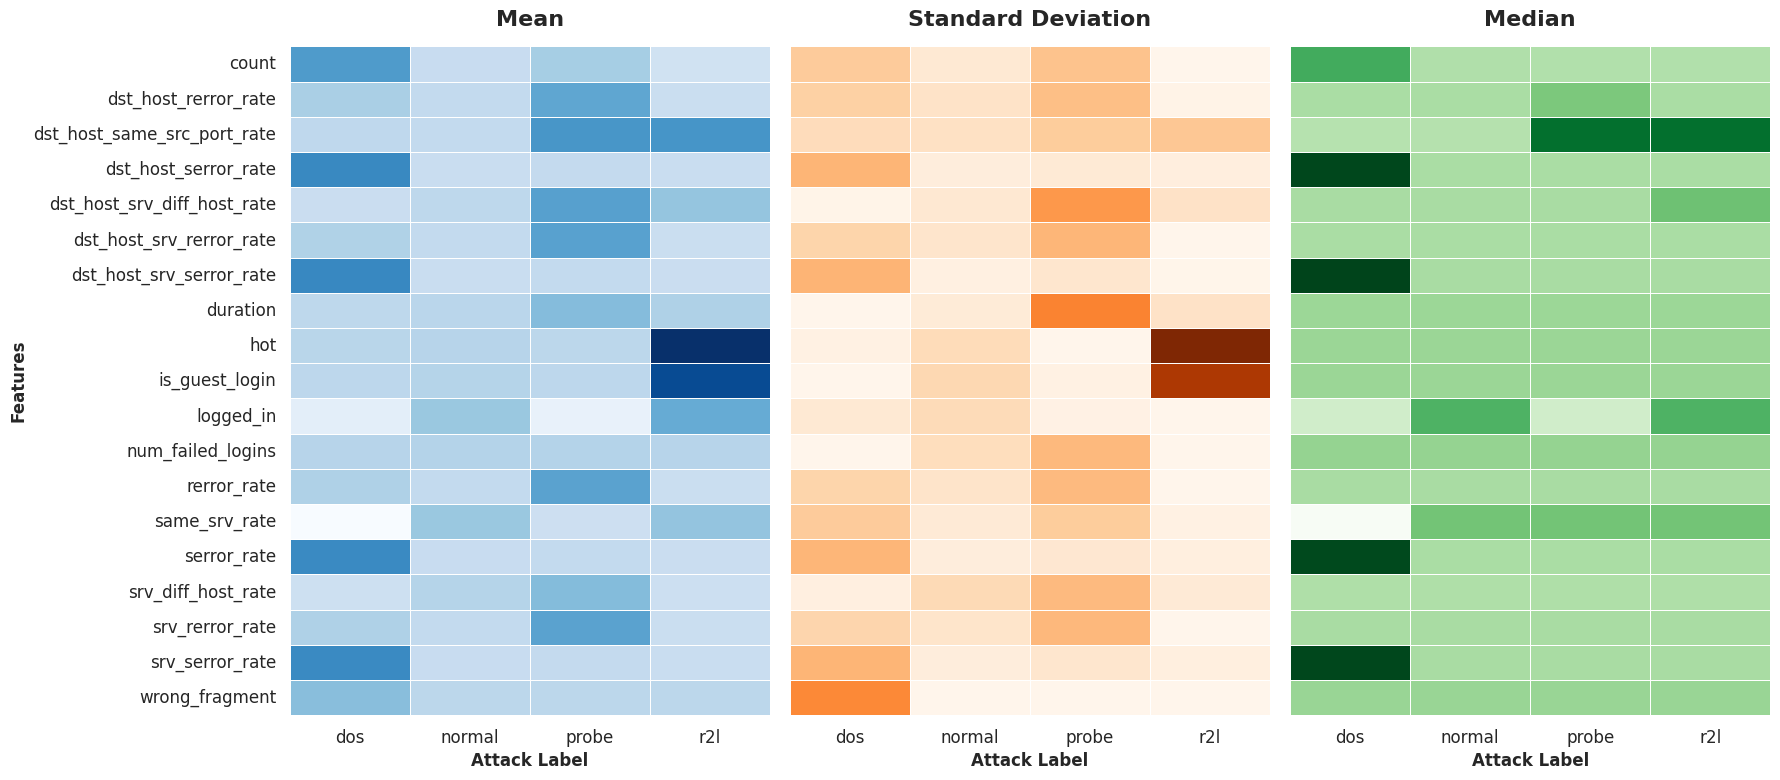
\includegraphics[width=\linewidth]{images/task1/task1_heatmaps_combined.png}
        \caption{Feature analysis across attack classes: standardized Mean, Standard Deviation, and Median. DoS attacks exhibit strong error-rate signals, while R2L attacks closely mimic normal traffic.}
        \label{fig:task1_heatmaps}
    \end{figure}

    \noindent
    The heatmaps reveal clear discriminative structure, highlighting key features that differentiate the traffic classes.
    \textbf{DoS attacks} exhibit extremely elevated \texttt{serror\_rate} and \texttt{srv\_serror\_rate} ($\mu > 2.0$ standard deviations above the global mean), reflecting SYN flood behavior, alongside high \texttt{count} and \texttt{srv\_count} values consistent with connection floods. Additionally, DoS attacks show a significant negative mean/median for \texttt{same\_srv\_rate}, indicating that attackers hit many different services rather than concentrating on a single service as is common in benign traffic, and elevated values for \texttt{wrong\_fragment} due to malformed packet transmission.
    \textbf{Probe attacks} are characterized by high \texttt{dst\_host\_srv\_diff\_host\_rate} and elevated service diversity metrics, reflecting systematic port and host scanning. They also display elevated values for \texttt{dst\_host\_same\_src\_port\_rate}, indicating systematic scanning from a single port. Notably, the medians for these features are considerably lower than their corresponding means, illustrating a highly skewed distribution driven by a few intense, extreme scanners.
    \textbf{R2L attacks} show only subtle signatures --- slightly elevated \texttt{hot} and \texttt{is\_guest\_login} --- but otherwise closely resemble normal traffic, explaining why they are the hardest class to detect.
    \textbf{Normal traffic} exhibits low, stable values across all anomaly-indicative features with moderate connection rates, and is uniquely characterized by high values in \texttt{logged\_in} and \texttt{service\_http}, which are the most distinctive signatures of benign, legitimate user activity.

% --- Feature Correlation Analysis ---
\subsection{Feature Correlation Analysis} \label{sec:correlation}

    To quantify feature redundancy, we computed the Pearson correlation matrix (unfortunately not shown here due to space constraints) on the numerical training features. % (\Cref{fig:task1_correlation}).
    Several feature groups exhibit near-perfect correlation (e.g., \texttt{serror\_rate} and \texttt{srv\_serror\_rate}: $r > 0.98$; \texttt{dst\_host\_serror\_rate} and \texttt{dst\_host\_srv\_serror\_rate}), confirming that the feature space contains significant redundancy.
    This motivates PCA-based dimensionality reduction in \Cref{sec:task3}.

    % \begin{figure}[H]
    %     \centering
    %     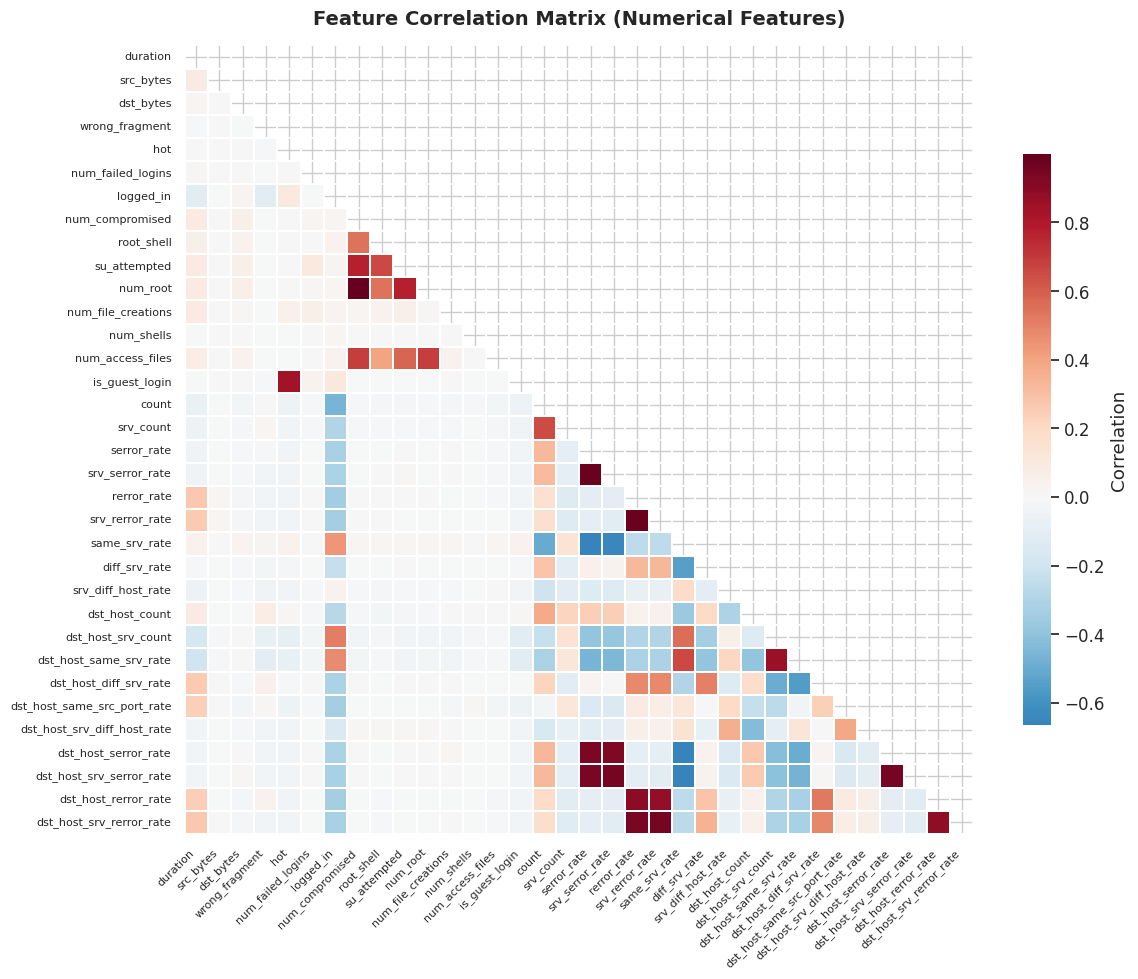
\includegraphics[width=0.85\linewidth]{images/task1/task1_correlation_matrix.png}
    %     \caption{Pearson correlation matrix of numerical features. Several traffic-rate and error-rate features are near-perfectly correlated, confirming high redundancy.}
    %     \label{fig:task1_correlation}
    % \end{figure}
